% mainfile: ../../../../master.tex
\subsection{MasterPure\texttrademark~ Complete DNA and RNA purification kit}
% The part of the label after the colon must match the file name. Otherwise,
% conditional compilation based on task labels does NOT work.
\label{task:20180201_cj4}
\tags{dna,rna,extr,lab}
\authors{cj}
%\files{}
%\persons{}

After I failed four times the simultaneous extraction of DNA and RNA based on Phenol pH 4, I want to attempt the extraction of DNA and RNA with the kit MasterPure\texttrademark.

% Figures
\begin{figure}[H] % position of the figure 
    \centering
    \caption{Selection of the micro-algae culture for DNA and RNA extraction.}
    \label{fig:20180201_mia_cultures_selected}
    \begin{subfigure}[b]{0.3\textwidth}
        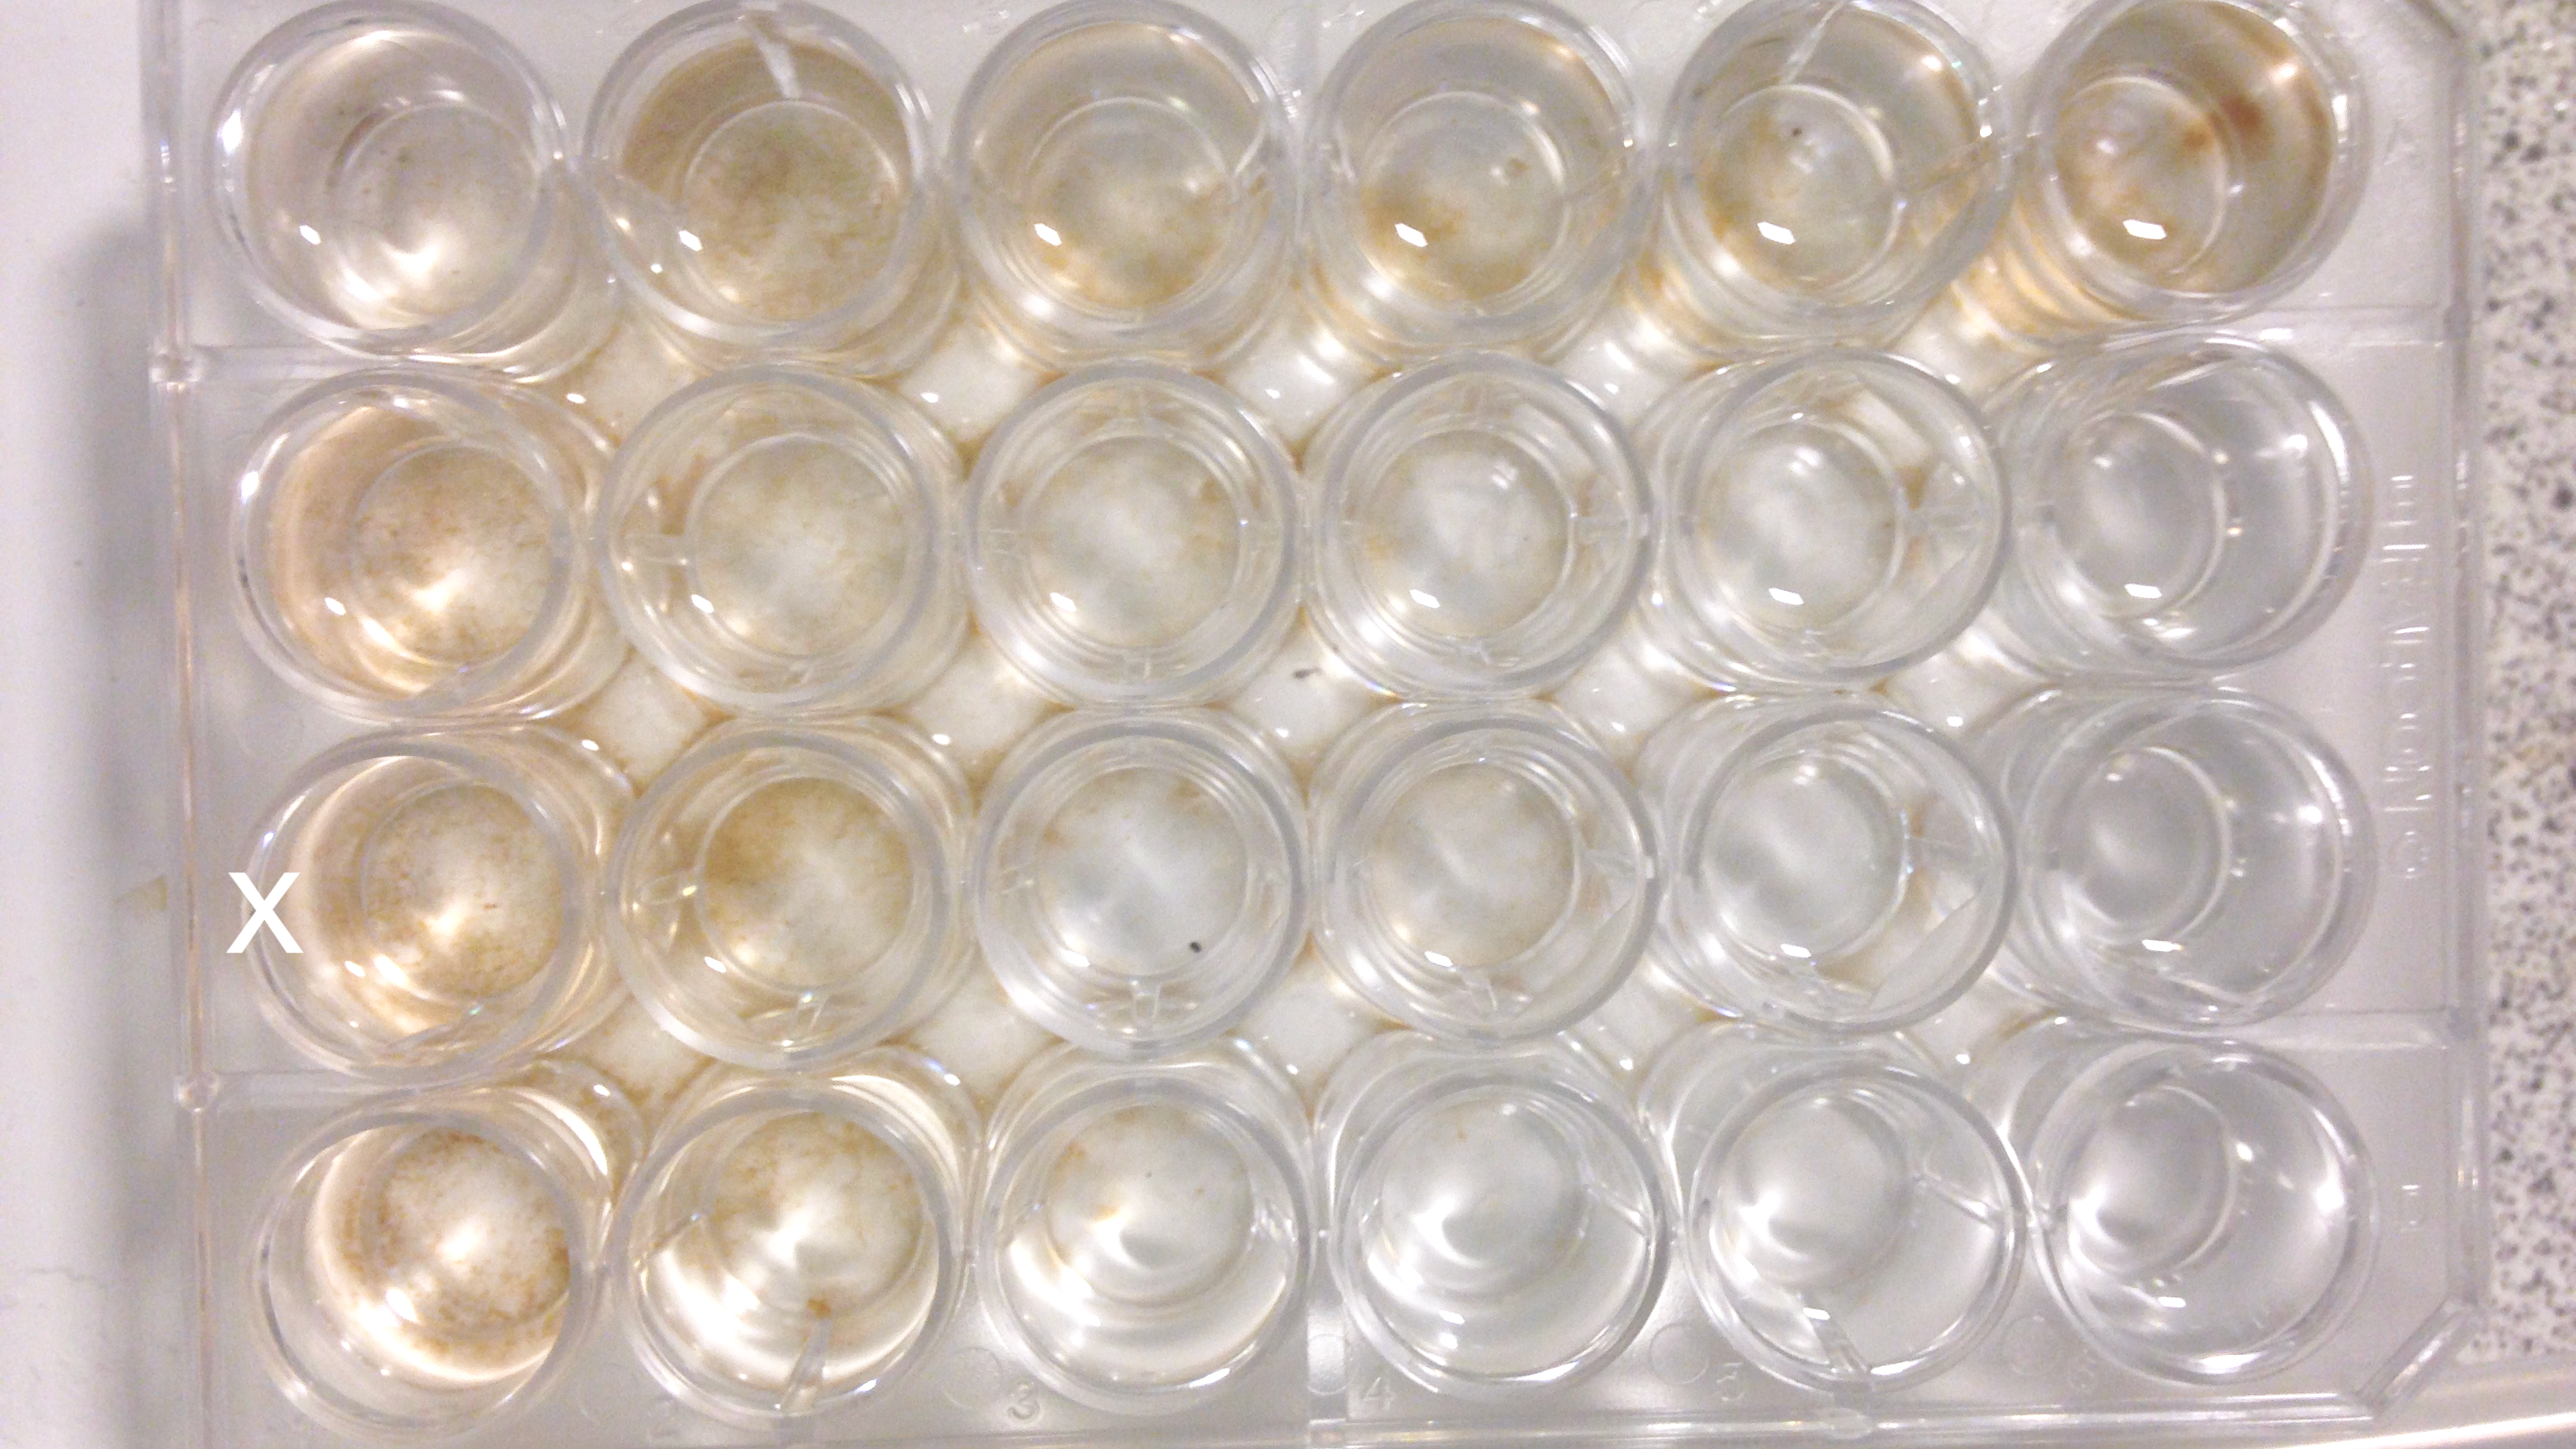
\includegraphics[width=\textwidth]{graphics/pic/20180201_mia_cultures1.png}
        \caption{Selected well labeled with X with sufficient growth}
        \label{sfig:20180201_mia_cultures1}
    \end{subfigure}
    ~ 
    \begin{subfigure}[b]{0.3\textwidth}
        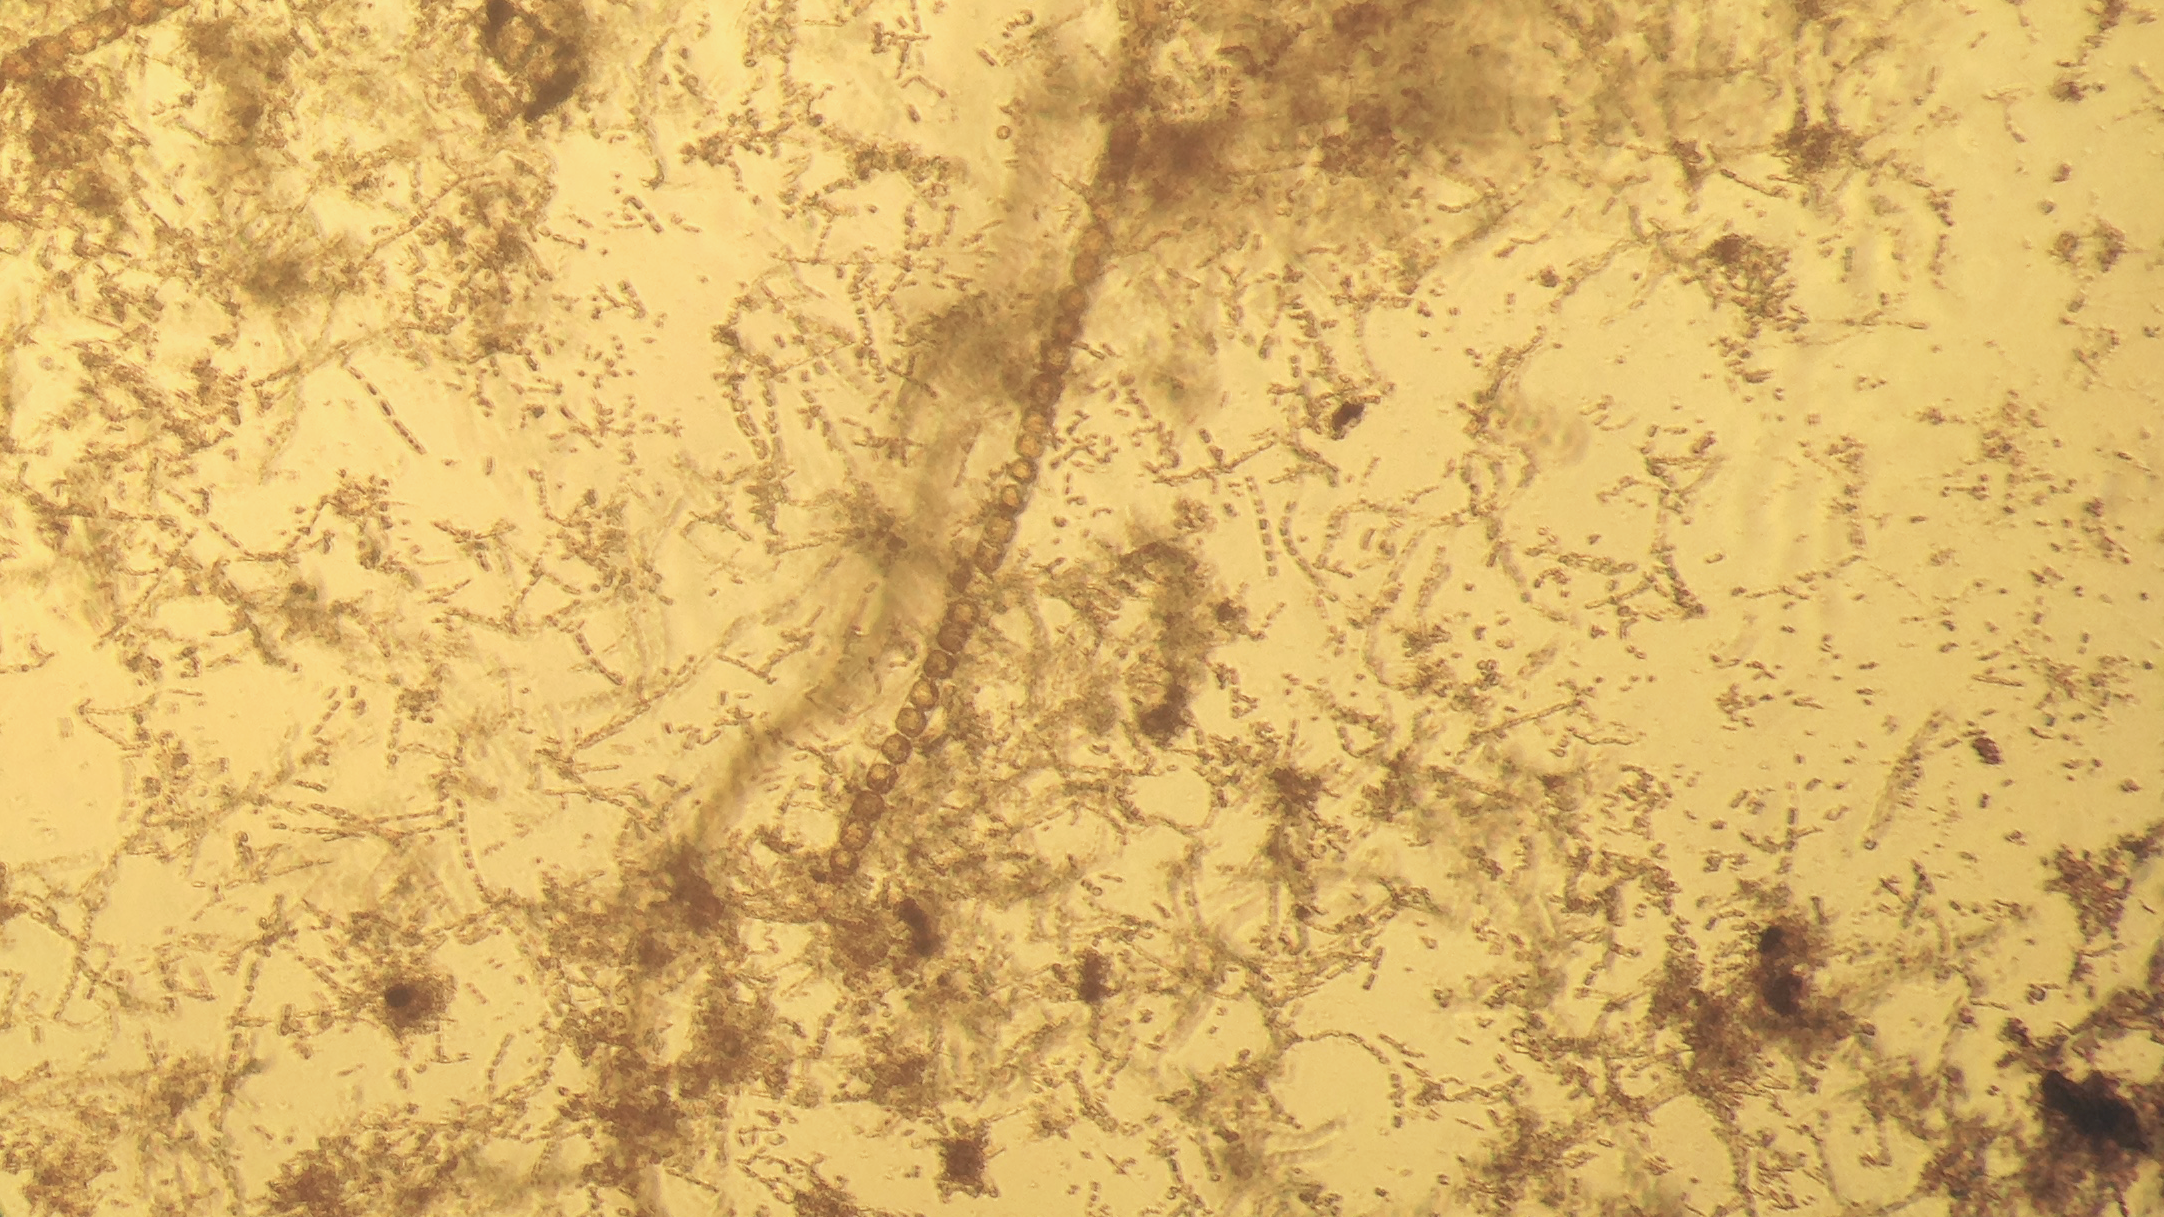
\includegraphics[width=\textwidth]{graphics/pic/20180201_mia_cultures_microscope.png}
        \caption{Picture of the culture under the microscope}
        \label{sfig:20180201_mia_cultures_microscope}
    \end{subfigure}
    ~ 
    \begin{subfigure}[b]{0.3\textwidth}
        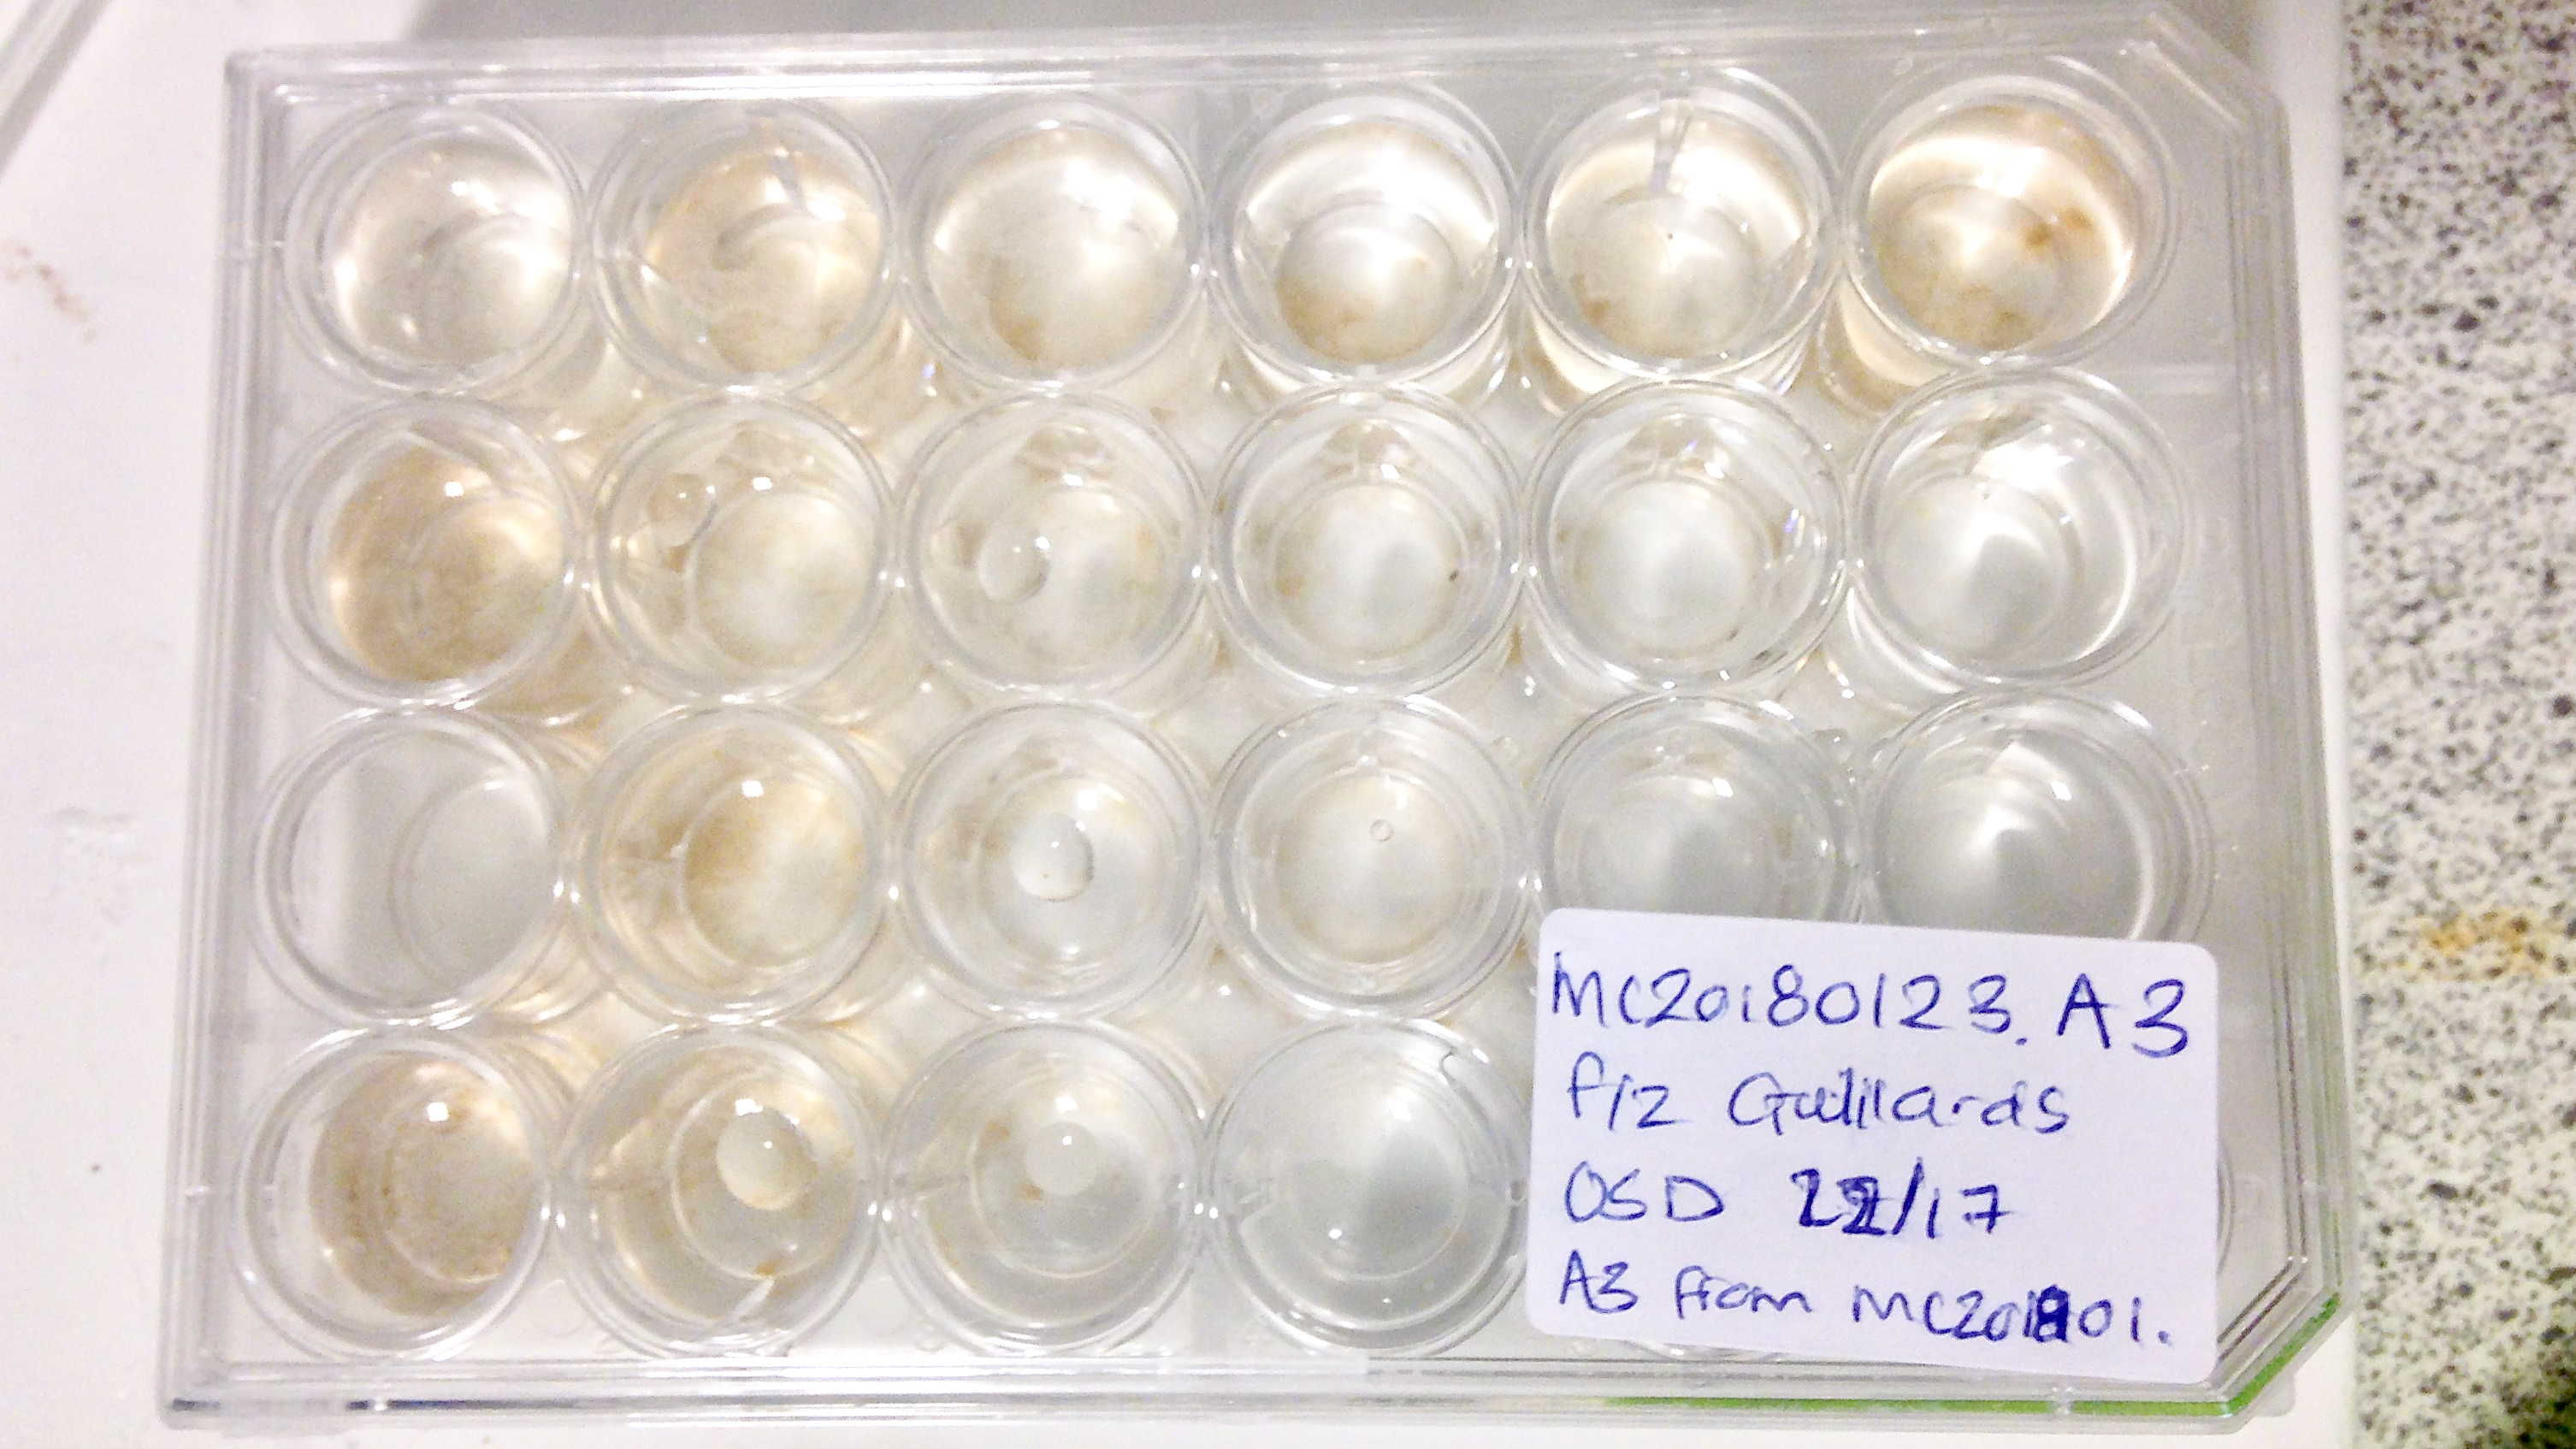
\includegraphics[width=\textwidth]{graphics/pic/20180201_mia_cultures.png}
        \caption{Plate after I took the about 2 mL of culture.}
        \label{sfig:20180201_mia_cultures}
    \end{subfigure}
\end{figure}

\begin{itemize}
\item Transfer about 2 mL of culture into a 2mL-Eppendorf tube with a pasteur pipette.
\item Pellet cells by centrifugation for 10 min at 8000 rpm at 4\degree C.
\item Discard carefully supernatent leaving approx. 25~\uL of liquid.
\comment{There was a lot more liquid left, but the pellet was very jelly-like.}
\end{itemize}


\subsubsection{Lysis of cells}

\begin{itemize}
\item Add 600~\uL of Tissue and cell lysis solution.
\item Add 1~\uL of Proteinase K.
\item Vortex for 10 sec.
\item Incubate at 65\degree C for 15 min (in hybrization over) and vortex every 5 min.
\item Place the sample on ice for 3-5 min and then proceed with the total nucleic acid precipitation.
\end{itemize}

\subsubsection{Precipitation of the Total Nucleic Acids}

\begin{itemize}
\item Add 150~\uL of MPC Protein Precipitation Reagent to the 600~\uL of lysed samples.
\item Vortex vigorously for 10 sec.
\item Pellet the debris by centrifugation at 4\degree C for 10 min at >10,000 g in a microcentrifuge. 
\comment{Here it was recommended to add an extra 25~\uL of MPC Protein Precipitation Reagent if the pellet was loose or clear, and I did not do it as I thought it was fine, but I should have done it.}
\item Transfer and split supernatent into two Eppendorf tubes and discard the pellet: one tube for DNA isolation and the second for RNA isolation.
\comment{Approximately 300~\uL in each tube.} 
\item Add 500~\uL of cold isopropanol to the recovered supernatent and invert 30-40 times (do this for both tubes).
\item Pellet nucleic acids by centrifugation at 4\degree C for 10 min at maximum speed in a microcentrifuge.
\item Proceed with RNA isolation.
\end{itemize}

\subsubsection{RNA isolation}

\begin{itemize}
\item Remove all supernatent without disturbing the pellet.
\item Prepare 200~\uL of DNase I solution by diluting 10~\uL of RNase-Free DNase I up to 200~\uL with 1 X DNase buffer.
\item Completely resuspend the total nucleic acids pellet in 200~\uL of DNase I solution.
\item Incubate at 37\degree C for 30 mine.
\comment{At this point, I keep on with the DNA isolation.}
\item Add 200~\uL of 2X Tissue and Cell Lysis Solution.
\item Vortex for 5 seconds.
\item Add 200~\uL of MPC Protein Precipitation Reagent.
\item Vortex 10 seconds.
\item Place on ice for 3-5 min.
\comment{Maybe on ice for longer as I was checking the gels with Mia.}
\item Pellet the debris by centrifugation for 10 min at 10000 x g in a microcentrifuge.
\item Transfer the supernatent containing the RNA into a clean microcentrifuge tube and discard the pellet.
\item Add 500\uL of isopropanol to the supernatent.
\item Invert tube 30-40 times.
\item Pellet the purified RNA by centrifugation at 4\degree C for 10 min.
\item Carefully pour off the isopropanol without dislodging the RNA pellet.
\item Rinse twice with 70\% ethanol being careful to not dislodge the pellet (Centrifuge briefly if the pellet is dislodged and remove all residual ethanol with a pipette).
\item Resuspend the RNA in 50~\uL of Tris-buffer.
\mistake{I don't know why I decided to use Tris buffer pH 8!!! I think I just did not think properly and did the same as I would have done with DNA, but RNA should be kept at slightly lower pH ... like in DEPC-treated water!}
\item Add 1~\uL of RiboGuard RNase Inhibitor.
\comment{At least I added the RiboGard in my NON-RNase FREE Tris buffer!}
\end{itemize}

\subsubsection{DNA isolation}

The nucleic acids should have been pelleted in isopropanol from previous steps.
\begin{itemize}
\item Carefully pour off the isopropanol without dislodging the pellet. 
\item Rinse twice with 70\% ethanol, being careful to not dislodge the pellet (Centrifuge briefly if the pellet is dislodged and remove all residual ethanol with a pipette).
\item Resuspend the DNA in 50~\uL of Tris-buffer.
\important{DO NOT USE TE BUFFER: it contains EDTA which inhibits PCR.}
\end{itemize}




